\chapter{Developping NeuroEvolution.jl}
\label{chap:neuroevo}

\href{https://github.com/TemplierPaul/NeuroEvolution.jl}{\color{blue}{NeuroEvolution.jl}} is a Julia library I developed to implement multiple neuroevolution algorithms for BERL. It includes \textbf{NEAT} (NEuroEvolution of Augmenting Topologies) and \textbf{HyperNEAT} Hypercube-based NEAT), and an implementation of a direct weights optimization in a fix network using \textbf{CMAES} (Covariance matrix adaptation evolution strategy) is in progress to complete it. 

The concepts powering the NEAT algorithm may seem relatively simple and clear as described in the literature, making it a quite elegant solution. \\
However, its implementation raises multiple complex issues, turning out to be rather intricate. The obstacles met when implementing part of it for an earlier \href{https://github.com/TemplierPaul/Genepy}{\color{blue}{personal project}},  and in the \href{https://github.com/d9w/NEAT.jl/tree/master/src}{\color{blue}{NEAT agent}} developed for the Breezy competition (cf chapter \ref{chap:dota}), helped design a more reliable structure and drastically reduced the development time.

This chapter aims at presenting the choices made during the design and development of NeuroEvolution.jl, its architecture and the main principles ruling it. 

\section{NEAT implementation}
I developed the NEAT algorithm based on the original papers \cite{NEAT_1} and \cite{NEAT_2}, taking into account the remarks and indications of the author on \href{https://www.cs.ucf.edu/~kstanley/neat.html#FAQ2}{
\color{blue}{his website}}. \\
The \href{https://github.com/FernandoTorres/NEAT}{\color{blue}{reorganized version}} of the original C++ implementation of NEAT also provided insight into the algorithm, although some parts were approached differently, taking the papers as reference.

\subsection{NEAT Individual}

Based on Cambrian.jl, NeuroEvolution.jl uses an abstract type \code{NEATIndiv} from which the structure \code{NEATIndividual} inherits. This allows to build new NEAT-like individuals using the same methods with additional features, like HyperNEAT which relies on the NEAT algorithm for evolution, but integrates a different evaluation procedure. \code{NEATIndiv} inherits from \code{Cambrian.Individual} to use Cambrian's architecture.

A \code{NEATIndividual} object contains a dictionary mapping an innovation number to a gene, which represents a connection between two neurons, a list of neurons defined by their positions, a dictionary mapping each neuron position to the activation function of the corresponding neuron, a \code{Network} object containing the neural network built from the genome, and a list of the fitness of the individual as required by Cambrian.

\begin{minipage}{\linewidth}
\begin{lstlisting}[language=Julia, caption=NEAT Individual (\href{https://github.com/TemplierPaul/NeuroEvolution.jl/blob/master/src/individual.jl}{\color{blue}{Source}})]
abstract type NEATIndiv <: Cambrian.Individual end

mutable struct NEATIndividual <: NEATIndiv
    genes::Dict
    fitness::Array{Float64}
    neuron_pos::Array{Float64}
    network::Network
    activ_functions::Dict
end
\end{lstlisting}
\end{minipage}

\subsection{Neuron position and Execution order}
\label{subsec:NEAT_neur_pos}

On of the main issues encountered when implementing NEAT in previous personal projects is the order of computation of the neurons. Due to the way it grows, the NEAT network can build recurrent connections, including bidirectional relationships with one connection from neuron A to neuron B, and one connection from B to A. Then, propagating depth from the output neurons to make sure all previous neuron values have been computed leads to an infinite loop between A and B, each one needing to be computed before the other. 

To prevent that issue and reduce the time needed to build the network, this implementation of NEAT was inspired by the work of \cite{wilson2018positionalcgp} in which the position of a CGP node is described as a floating point value. The execution order is then available by design since they can be executed sequentially based on their positions. Recurrent connections are defined by destination neurons being before origins, which makes possible to allow or block them easily at mutation. 

This representation also removes the propagation time concept, making the NEAT network closer to standard neural networks. 

The position of a neuron is defined as follows:
\begin{itemize}
    \item All input neurons are placed with negative integer positions.  
    \item The bias neuron (constant equal to 1) is placed at $0$.  
    \item All output neurons are placed at positive integer positions, starting at $1$.
    \item All other neurons are placed with positions in $]0, 1[$.
\end{itemize}

\begin{figure}[H]
\centering
\captionsetup{justification=centering,margin=2cm}
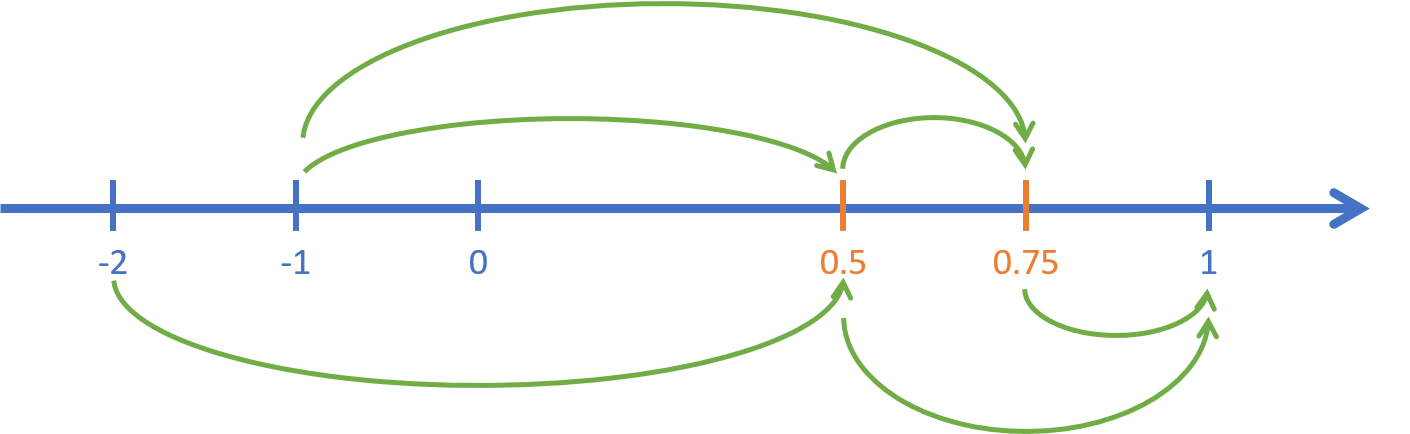
\includegraphics[width=10cm]{images/NEAT_position.png}
\caption{Example of NEAT individual as neurons defined by position and feed-forward connections, with 2 input features, 1 output neuron and 2 hidden neurons.}
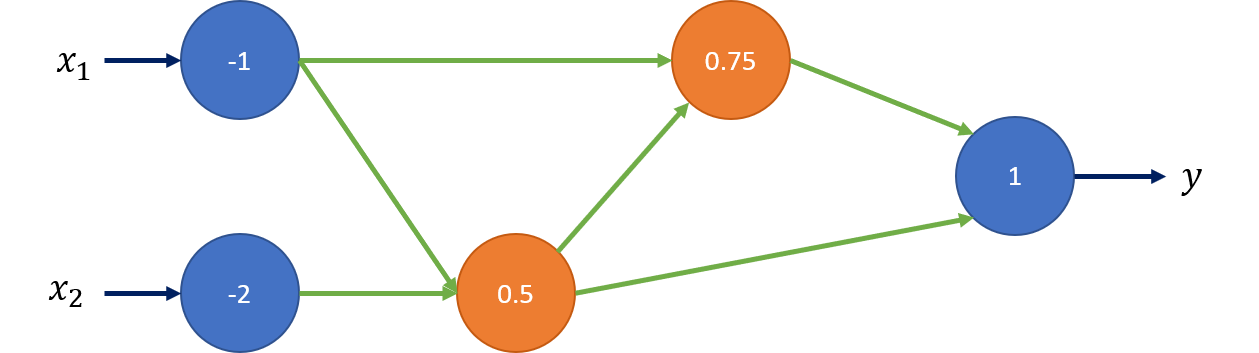
\includegraphics[width=10cm]{images/NEAT_network.png}
\caption{Neural Network generated from the above individual.}
 \label{NEAT_network}
\end{figure}

Neurons added through mutation of a connection are placed at a random position between the origin node of the connection at $p_o$ and the destination node at $p_d$, so that the order of execution is not modified. \\
The position of the new neuron is therefore randomly drawn in $]p_o, p_d[ \: \cap \: ]0, 1[$.

Because of this structure, and to avoid edge cases, connections between 2 output neurons are forbidden. Connections towards input and bias neurons are blocked too, since their values are fixed to the input vector and to 1 respectively.

When computing the network's output, its neurons are sorted by ascending position. Since the position determines the neuron type, choosing the update type is simple:

\begin{minipage}{\linewidth}
\begin{lstlisting}[language=Julia, caption=NEAT network processing (\href{https://github.com/TemplierPaul/NeuroEvolution.jl/blob/master/src/process.jl}{\color{blue}{Source}})]
for p in indiv.neuron_pos
    if p < 0 # Input neurons
        indiv.network.neurons[p].output = 
                    last_features[Int(-p)]
    elseif p == 0 # Bias neuron
        indiv.network.neurons[p].output = 1
    else # Hidden and output neurons
        compute!(indiv.network.neurons[p], 
                    indiv.network.neurons)
    end
end
\end{lstlisting}
\end{minipage}

\subsection{Run configuration}

The parameters to run NEAT are defined in a \href{https://github.com/TemplierPaul/NeuroEvolution.jl/blob/master/cfg/test.yaml}{\color{blue}{YAML file}}  that is read at runtime. It includes:

\begin{itemize}
    \item Cambrian settings: population size, number of generations
    \item Input and output size of the network
    \item Speciation parameters
    \item Mutation probabilities for each mutation type
    \item Available activation functions including sigmoid, trigonometric functions, absolute value, identity, or ReLU. 
\end{itemize}

One of the available activation functions is randomly selected when a new neuron is created, allowing the implementation of a Compositional Pattern-Producing Network (CPPN) by making multiple ones available. The default activation function for NEAT is the sigmoid. 

\subsection{Crossover and innovation number}
A usually delicate part of the implementation of NEAT lies in the management of the innovation number, which tracks genes across the population and guarantees the same gene is recognized on both sides during crossover.

In this implementation, and according to Cambrian's structure, a configuration dictionary is passed across the algorithm to each method requiring run parameters, built from the YAML configuration file. The innovation number is stored inside and updated after each mutation adding a gene. 

Using a dictionary in the individual to store each gene linked to its innovation number allows to compare genomes more efficiently at crossover than an array of genes. 

\subsection{Speciation threshold}
NEAT relies on speciation to update its population:
\begin{itemize}
    \item If individuals are closer than the speciation threshold, they get put in the same species
    \item The fitness of each individual is computed with explicit fitness sharing, hence divided by the size of the population of their species
    \item Offspring are distributed among species depending on the mean (or the max) fitness in the current members of the species
    \item Reproduction is computed in each species by selecting parents randomly in the top members of the species (or based on their individual fitness in a tournament selection) and applying either mutation or crossover.
    \item All offspring are assigned to the closest species
\end{itemize}

However as generations occur the distance between genomes grows and the algorithm tends to assign a different species to each individual, hence causing hundreds of species to appear. In order to keep a stable number of species, K.O.Stanley introduces on his website a changing threshold, increasing of decreasing by a fix amount in order to keep the number of active species stable. 

I introduced a slightly modified version of this algorithm as \code{update\_threshold!}, which modifies the threshold by an amount scaled on the ratio: $$current\_species\_number \over wanted\_species\_number$$

This solution yields a very stable number of species, although usually higher than the wanted number.

\subsection{NEAT in a standard Genetic Algorithm}

The goal of using Cambrian as a framework in this implementation also was to allow for a high compatibility with other algorithm so that the coding blocks defined for NEAT could be reused in classical evolutionary algorithms, from a Genetic Algorithm (GA) to a Quality-Diversity method as envisioned in the Breezy competition (cf chapter \ref{chap:dota}). 

Hence, I finally implemented a simple wrapper to use the NEAT Individual and its mutation and crossover operators in a standard Genetic Algorithm, ignoring the specific species-based populate function for the standard Cambrian \code{ga\_populate} function.

\begin{minipage}{\linewidth}
\begin{lstlisting}[language=Julia, caption=Genetic Algorithm populate for NEAT  (\href{https://github.com/TemplierPaul/NeuroEvolution.jl/blob/master/src/evolution.jl}{\color{blue}{Source}})]
function neat_ga_populate!(e::Evolution)
    mut::Function=i::NEATIndiv -> 
                    NeuroEvolution.mutate(i, e.cfg)
    cross::Function=(p1, p2) -> 
                    NeuroEvolution.crossover(p1, p2, e.cfg)
    Cambrian.ga_populate!(e, mutation=mut, crossover=cross)
end
\end{lstlisting}
\end{minipage}

This compatibility with other Cambrian algorithms allows to easily use the NEAT individual in other settings such as Quality-Diversity methods or open-ended evolution, thus helping in new algorithms research.

\section{Adding HyperNEAT}
HyperNEAT \cite{HyperNEAT} introduces indirect encoding by using a CPPN (Compositional Pattern-Producing Network \cite{CPPN}) to determine the weights of a neural network with a fix architecture. Since the CPPN can be evolved with the NEAT algorithm for HyperNEAT, most evolutionary methods in NeuroEvolution.jl can be reused. \\ 
However, instead of evaluating the evolved network (the CPPN) to solve the problem, the CPPN is used to determine the weights of a network with fixed architecture, referenced here as the \code{final network}. 

\subsection{HyperNEAT Individual}

HyperNEAT was added to NeuroEvolution.jl by creating a structure \code{HyperNEATIndiv}, inheriting from \code{NEATIndividual} like \code{NEATIndiv}. Thus, functions affecting the evolved network (e.g. mutation, crossover, populate) take as arguments any object inheriting from the abstract type \code{NEATIndividual}, and are blind to whether NEAT or HyperNEAT is used. Conversely, other functions related to the evaluation of an individual (e.g. evaluate, build, process) are algorithm-specific and are defined for each individual type.

\begin{minipage}{\linewidth}
\begin{lstlisting}[language=Julia, caption=HyperNEAT Individual (\href{https://github.com/TemplierPaul/NeuroEvolution.jl/blob/master/src/HyperNEAT.jl}{\color{blue}{Source}})]
mutable struct HyperNEATIndividual <: NEATIndiv
    genes::Dict
    fitness::Array{Float64}
    neuron_pos::Array{Float64}
    network::Network
    activ_functions::Dict
    hn_net::GridNetwork
end
\end{lstlisting}
\end{minipage}

\code{HyperNEATIndividual} uses the same structure as \code{NEATIndividual}, adding a \code{hn\_network} field to store the generated final network described in subsection \ref{sub:final-hn-net}.

\subsection{Final network definition}
\label{sub:final-hn-net}
The final network is a feed-forward, fully-connected neural network with a fixed architecture. It is build from an array of \code{Layer} objects, each containing the output values of a neurons layer, and an array of \code{Connection} objects linking 2 layers and implementing weights. 

\begin{minipage}{\linewidth}
\begin{lstlisting}[language=Julia, caption=HyperNEAT final network (\href{https://github.com/TemplierPaul/NeuroEvolution.jl/blob/master/src/HyperNEAT.jl}{\color{blue}{Source}})]
mutable struct GridNetwork
    layers::Array{Layer}
    connections::Array{Connection}
end
\end{lstlisting}
\end{minipage}

The \code{build!} method creates the final network and sets its weighs with the CPPN, while the \code{process!} method computes the output of the final network. This approach allows to only build the network once, but increases complexity by adding a step to place between mutation and evaluation.

\subsection{Run configuration}

Using HyperNEAT requires a \href{https://github.com/TemplierPaul/NeuroEvolution.jl/blob/master/cfg/hyperneat.yaml}{\color{blue}{specific YAML file}} which adds information about hidden layers and structure of the generated network to the standard NEAT parameters. 

Although the default architecture for the final networks only links a layer of neurons to the previous one, toggling the \code{hn\_link\_all\_layers} parameter to \code{true} creates a connection between each layer and all the previous ones, for a more complex architecture. Using a CPPN for weights generation makes it possible to use such architecture without expanding the search space, contrary to direct encoding. 

\section{CMA-ES applied to neuroevolution}

%%% Local Variables: 
%%% mode: latex
%%% TeX-master: "isae-report-template"
%%% End: 